\section{Qualitative Analysis}
\label{sec:qualitative_analysis}

We present qualitative comparisons of our UniCL-AffSeg framework against the WeCLIP baseline and ground truth annotations on selected Pascal VOC 2012 images. Both class activation maps (CAMs) and pseudo-labels are visualized to highlight differences in object localization, boundary delineation, and overall mask quality.

% \subsection{Selection of Examples}
% The images were chosen to represent a variety of scenarios, including: 
% \begin{itemize}
%     \item \t	\textbf{Easy cases:} Large, isolated objects where CAMs are expected to cover most of the object region.
%     \item \t	\textbf{Challenging cases:} Small objects, occlusions, or cluttered backgrounds where weakly supervised CAMs often fail to capture complete object extents.
% \end{itemize}

% \subsection{Visualization Layout}
% Figure~\ref{fig:qualitative_comparison} shows the qualitative results in a structured grid. 
% The first row presents the input image, ground truth, WeCLIP CAM, and our CAM, while the second row shows the corresponding pseudo-labels generated by WeCLIP and our method. This layout allows a direct comparison of both intermediate activations and the resulting segmentation masks.


\begin{figure}[ht]
  \centering
  \setlength{\tabcolsep}{2pt} % adjust spacing
  \renewcommand{\arraystretch}{0.9}

  % Wrap the table in a colored box (requires \usepackage{tcolorbox})
  \begin{tcolorbox}[colframe=black!60, colback=white, boxrule=0.8pt, arc=2pt, left=2pt, right=2pt, top=2pt, bottom=2pt]
    \centering
    % CAMs with class labels on the left
    \begin{tabular}{m{3cm} c c c} % first column = label

      % Column headers
       & (a) Input                                                    & (b) WeCLIP & (c) Ours
      \\
      [1mm]

      {\textbf{Cat}}
       & 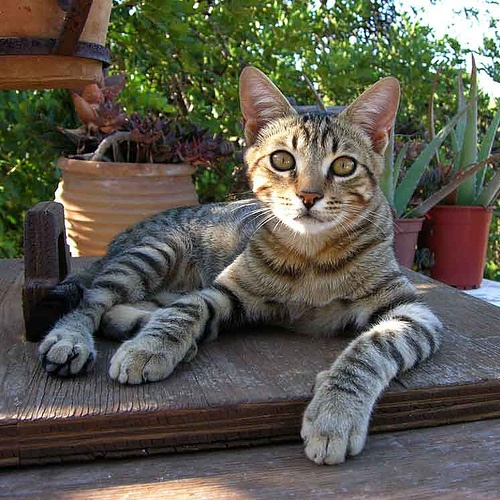
\includegraphics[width=0.20\textwidth,height=0.20\textwidth]
      {figures/originals/2007_003778}
       & 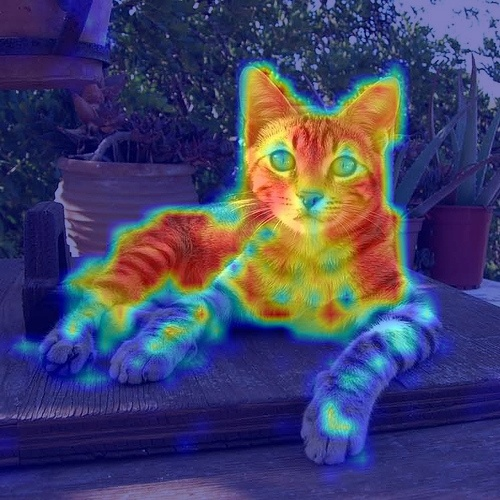
\includegraphics[width=0.20\textwidth,height=0.20\textwidth]
      {figures/val_cams/weclip/2007_003778_7}
       & 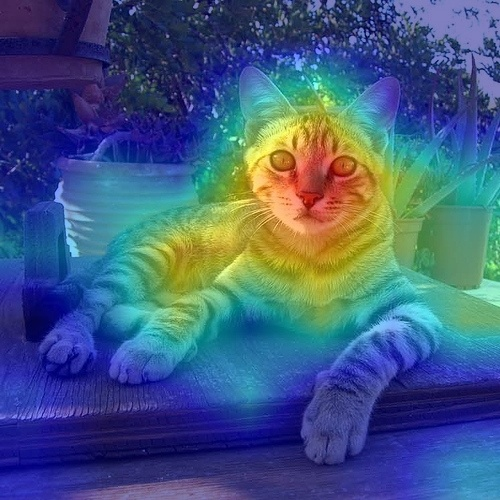
\includegraphics[width=0.20\textwidth,height=0.20\textwidth]
      {figures/val_cams/ours/2007_003778_7}
      \\
      \textbf{Bicycle}
       & 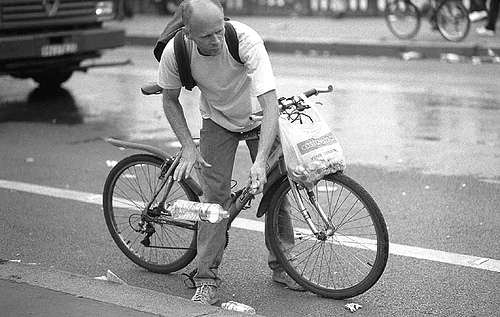
\includegraphics[width=0.20\textwidth,height=0.20\textwidth]
      {figures/originals/2011_000453}
       & 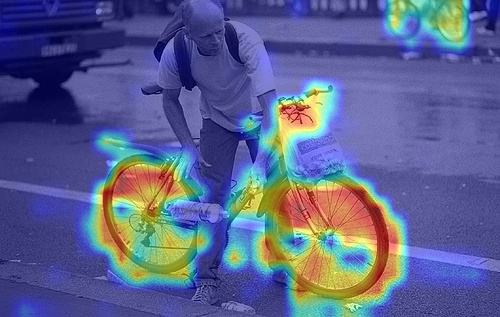
\includegraphics[width=0.20\textwidth,height=0.20\textwidth]
      {figures/val_cams/weclip/2011_000453_1}
       & 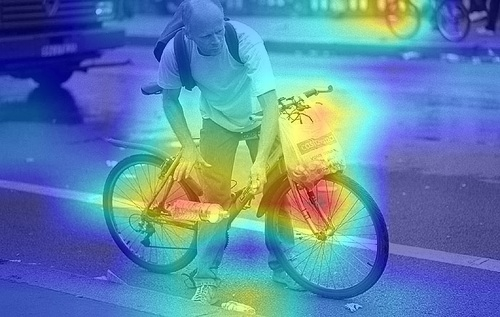
\includegraphics[width=0.20\textwidth,height=0.20\textwidth]
      {figures/val_cams/ours/2011_000453_1}
      \\
      \textbf{Bird}
       & 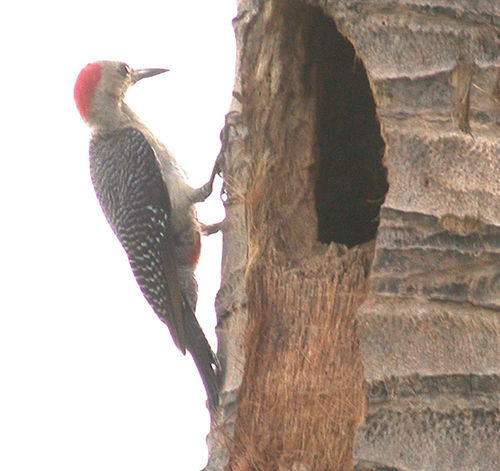
\includegraphics[width=0.20\textwidth,height=0.20\textwidth]
      {figures/originals/2011_001902}
       & 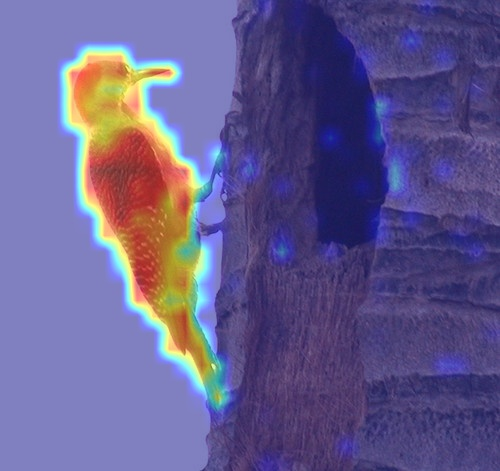
\includegraphics[width=0.20\textwidth,height=0.20\textwidth]
      {figures/val_cams/weclip/2011_001902_2}
       & 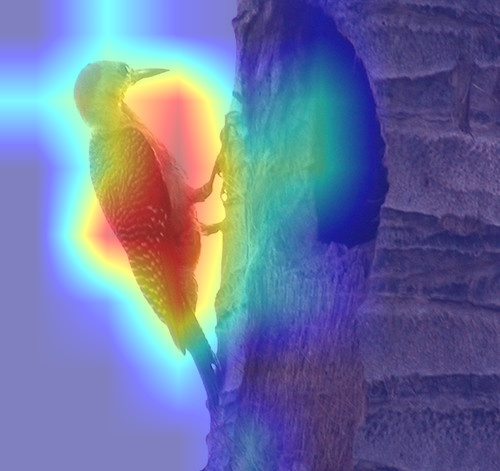
\includegraphics[width=0.20\textwidth,height=0.20\textwidth]
      {figures/val_cams/ours/2011_001902_2}
      \\
      \textbf{Boat}
       & 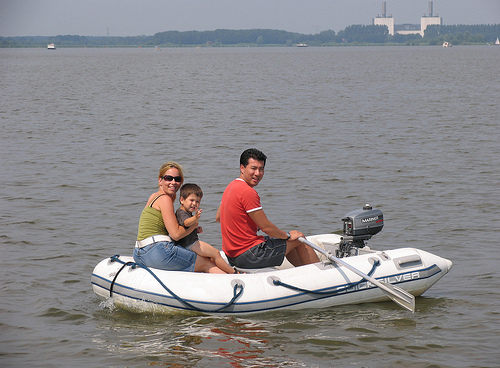
\includegraphics[width=0.20\textwidth,height=0.20\textwidth]
      {figures/originals/2010_003599}
       & 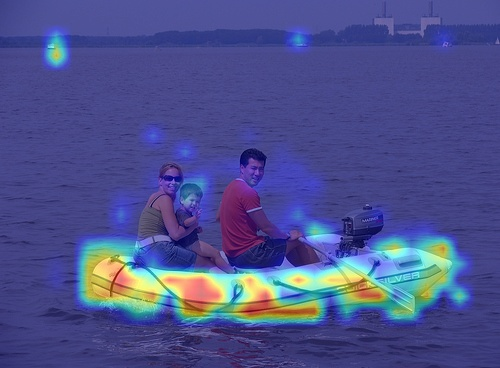
\includegraphics[width=0.20\textwidth,height=0.20\textwidth]
      {figures/val_cams/weclip/2010_003599_3}
       & 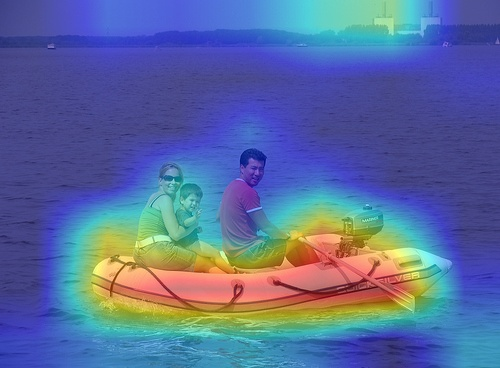
\includegraphics[width=0.20\textwidth,height=0.20\textwidth]
      {figures/val_cams/ours/2010_003599_3}
      \\
      \textbf{Pottedplant}
       & 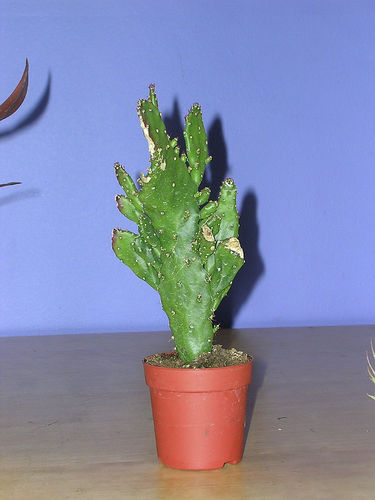
\includegraphics[width=0.20\textwidth,height=0.20\textwidth]
      {figures/originals/2011_000145}
       & 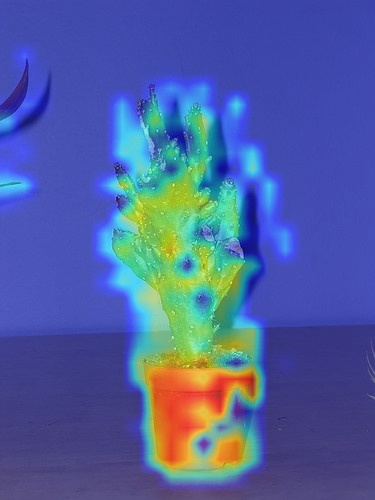
\includegraphics[width=0.20\textwidth,height=0.20\textwidth]
      {figures/val_cams/weclip/2011_000145_15}
       & 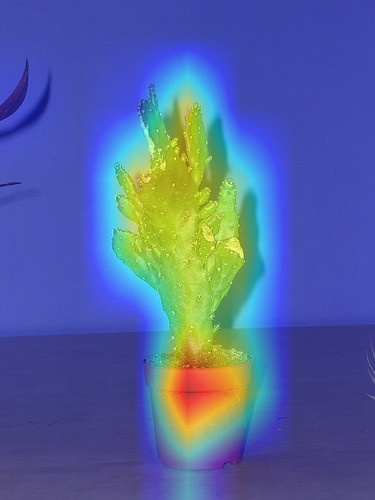
\includegraphics[width=0.20\textwidth,height=0.20\textwidth]
      {figures/val_cams/ours/2011_000145_15}
      \\
      \textbf{Car}
       & 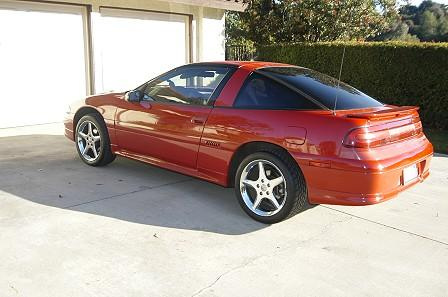
\includegraphics[width=0.20\textwidth,height=0.20\textwidth]
      {figures/originals/2010_005119}
       & 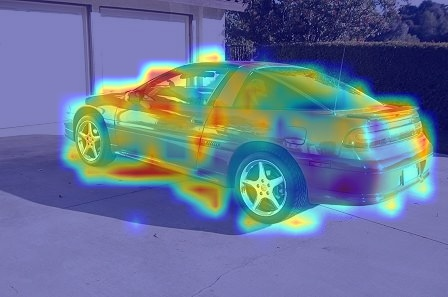
\includegraphics[width=0.20\textwidth,height=0.20\textwidth]
      {figures/val_cams/weclip/2010_005119_6}
       & 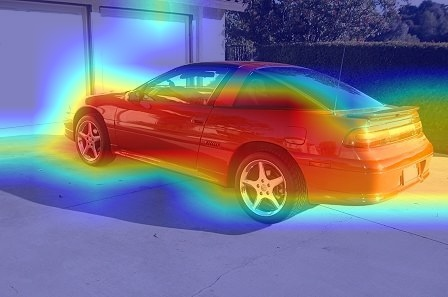
\includegraphics[width=0.20\textwidth,height=0.20\textwidth]
      {figures/val_cams/ours/2010_005119_6}
      \\
      \textbf{Bus}
       & 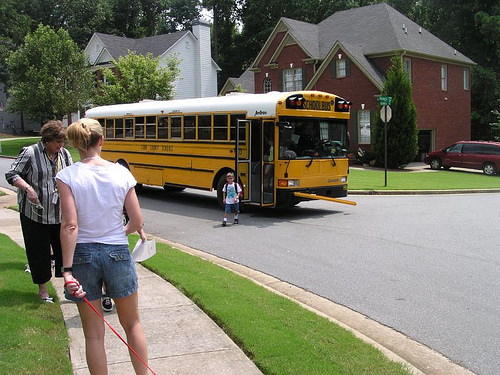
\includegraphics[width=0.20\textwidth,height=0.20\textwidth]
      {figures/originals/2010_000148}
       & 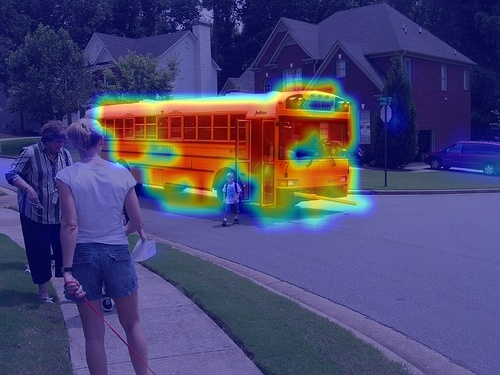
\includegraphics[width=0.20\textwidth,height=0.20\textwidth]
      {figures/val_cams/weclip/2010_000148_5}
       & 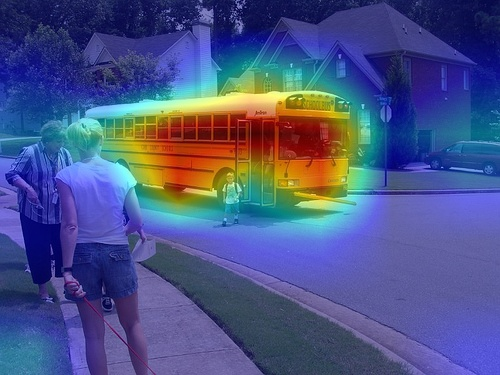
\includegraphics[width=0.20\textwidth,height=0.20\textwidth]
      {figures/val_cams/ours/2010_000148_5}
      \\
    \end{tabular}
  \end{tcolorbox}

  \caption{Qualitative comparison of CAMs between WeCLIP and our UniCL-AffSeg on PASCAL VOC 2012 \textit{val} set.}
  \label{fig:qualitative_comparison_cam_val}
\end{figure}


\begin{figure}[ht]
  \centering
  \setlength{\tabcolsep}{2pt} % adjust spacing
  \renewcommand{\arraystretch}{0.9}
  % Wrap the table in a colored box (requires \usepackage{tcolorbox})
  \begin{tcolorbox}[colframe=black!60, colback=white, boxrule=0.8pt, arc=2pt, left=2pt, right=2pt, top=2pt, bottom=2pt]
    \centering
    \begin{tabular}{cccc}
      (a) Input & (b) GT & (c) WeCLIP & (d) Ours           \\
      [1mm]

      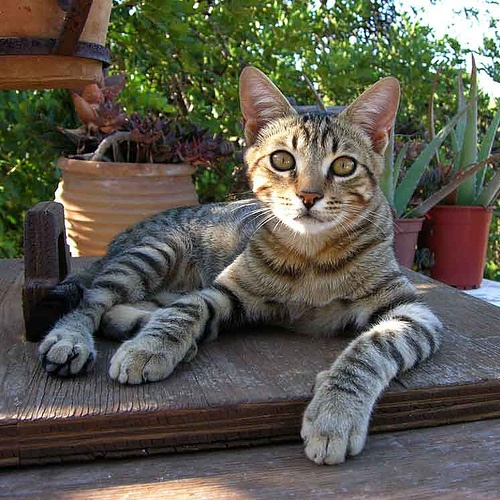
\includegraphics[width=0.20\textwidth,height=0.20\textwidth]
      {figures/originals/2007_003778}
                &
      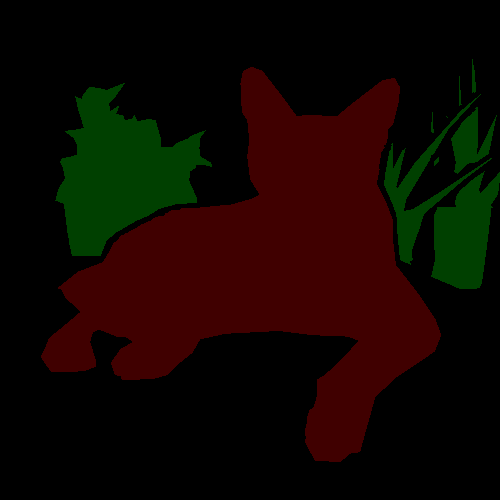
\includegraphics[width=0.20\textwidth,height=0.20\textwidth]
      {figures/colored_gts/2007_003778}
                &
      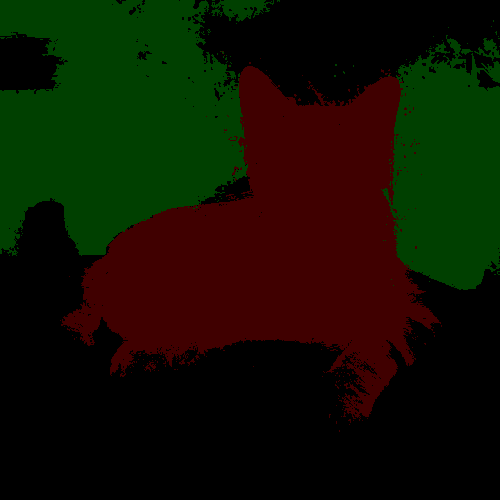
\includegraphics[width=0.20\textwidth,height=0.20\textwidth]
      {figures/val_labels/weclip/2007_003778_[7, 15]}
                &
      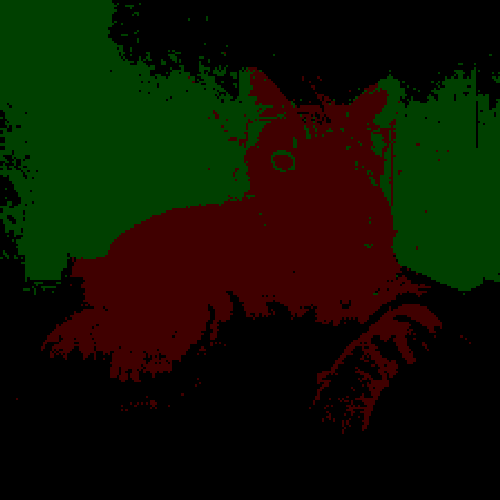
\includegraphics[width=0.20\textwidth,height=0.20\textwidth]
      {figures/val_labels/ours/2007_003778_[7, 15]}    \\

      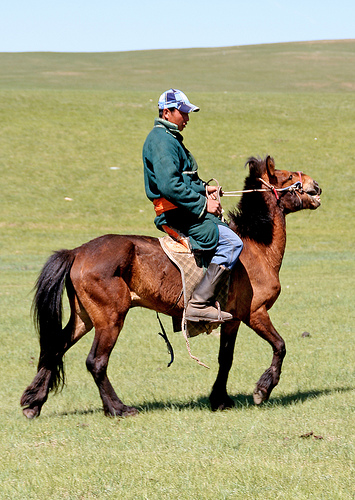
\includegraphics[width=0.20\textwidth,height=0.20\textwidth]
      {figures/originals/2009_003768}
                &
      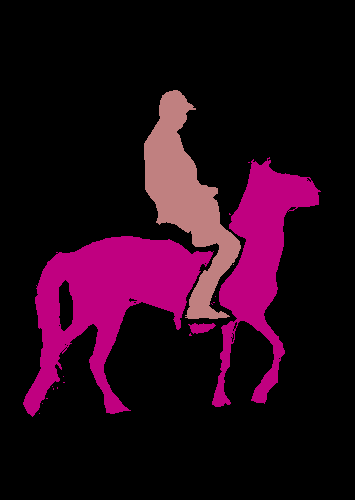
\includegraphics[width=0.20\textwidth,height=0.20\textwidth]
      {figures/colored_gts/2009_003768}
                &
      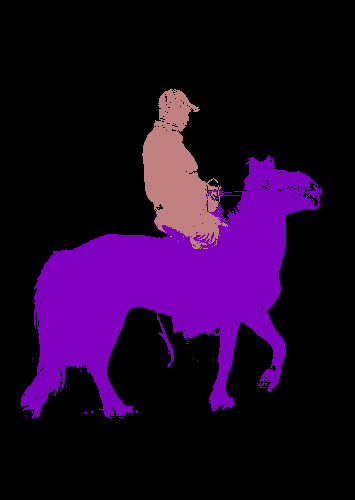
\includegraphics[width=0.20\textwidth,height=0.20\textwidth]
      {figures/val_labels/weclip/2009_003768_[12, 14]}
                &
      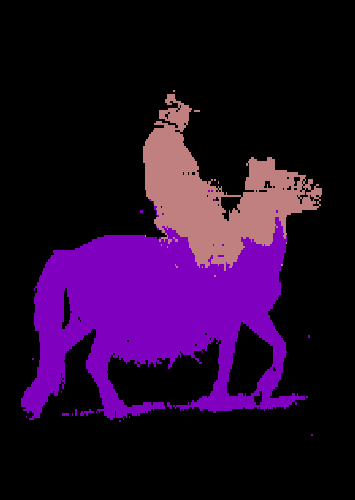
\includegraphics[width=0.20\textwidth,height=0.20\textwidth]
      {figures/val_labels/ours/2009_003768_[12, 14]}   \\

      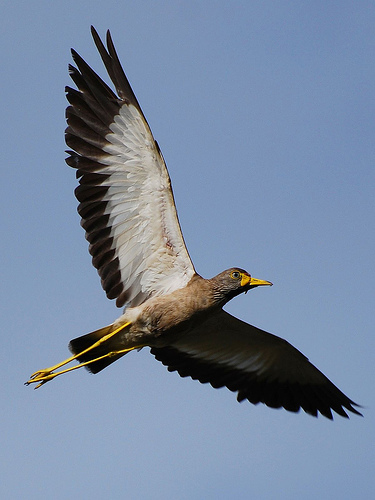
\includegraphics[width=0.20\textwidth,height=0.20\textwidth]
      {figures/originals/2011_001967}
                &
      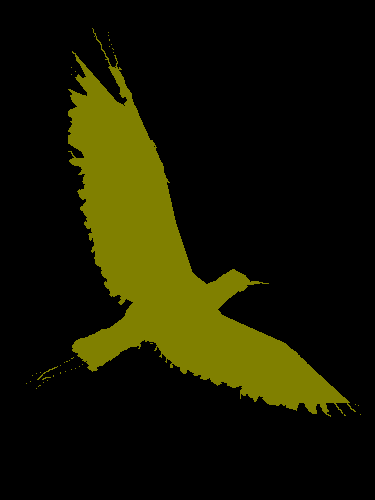
\includegraphics[width=0.20\textwidth,height=0.20\textwidth]
      {figures/colored_gts/2011_001967}
                &
      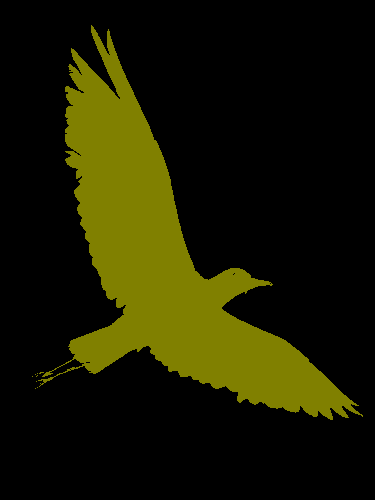
\includegraphics[width=0.20\textwidth,height=0.20\textwidth]
      {figures/val_labels/weclip/2011_001967_[2]}
                &
      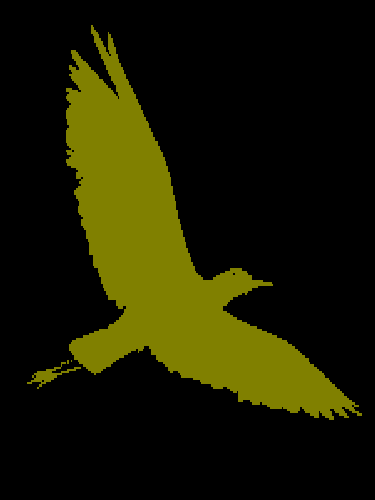
\includegraphics[width=0.20\textwidth,height=0.20\textwidth]
      {figures/val_labels/ours/2011_001967_[2]}        \\


      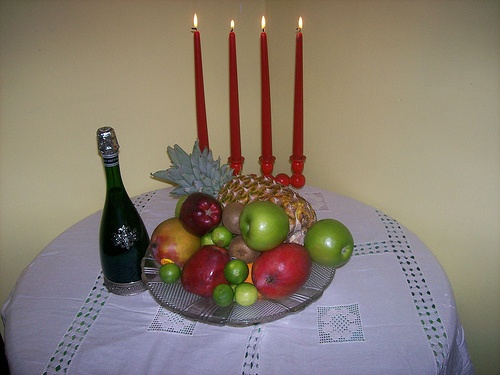
\includegraphics[width=0.20\textwidth,height=0.20\textwidth]
      {figures/originals/2007_000250}
                &
      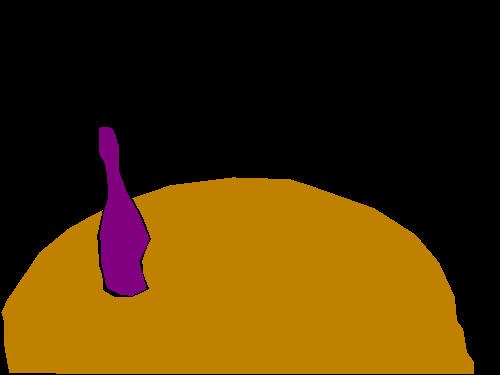
\includegraphics[width=0.20\textwidth,height=0.20\textwidth]
      {figures/colored_gts/2007_000250}
                &
      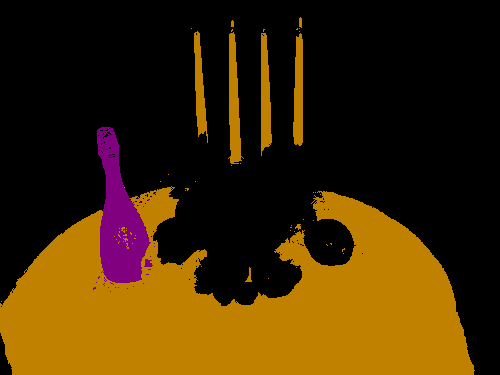
\includegraphics[width=0.20\textwidth,height=0.20\textwidth]
      {figures/val_labels/weclip/2007_000250_[4, 10]}
                &
      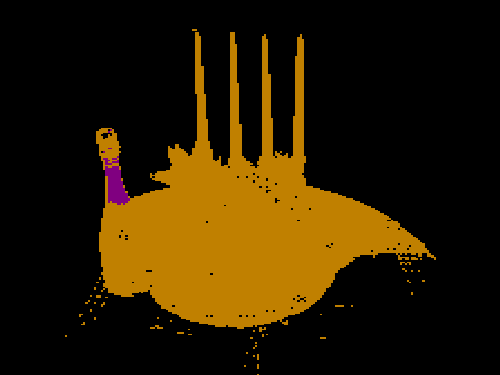
\includegraphics[width=0.20\textwidth,height=0.20\textwidth]
      {figures/val_labels/ours/2007_000250_[4, 10]}    \\


      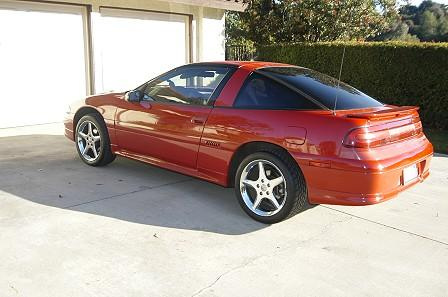
\includegraphics[width=0.20\textwidth,height=0.20\textwidth]
      {figures/originals/2010_005119}
                &
      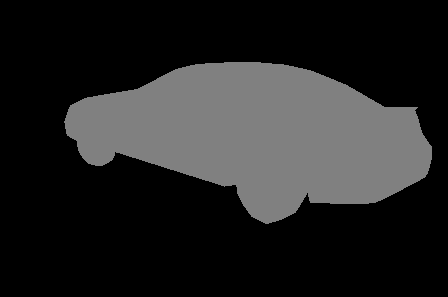
\includegraphics[width=0.20\textwidth,height=0.20\textwidth]
      {figures/colored_gts/2010_005119}
                &
      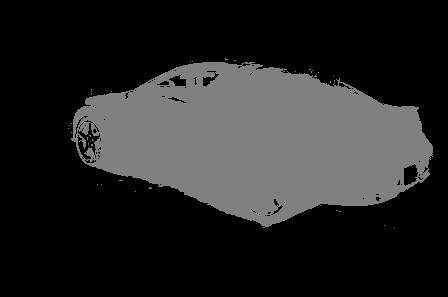
\includegraphics[width=0.20\textwidth,height=0.20\textwidth]
      {figures/val_labels/weclip/2010_005119_[6]}
                &
      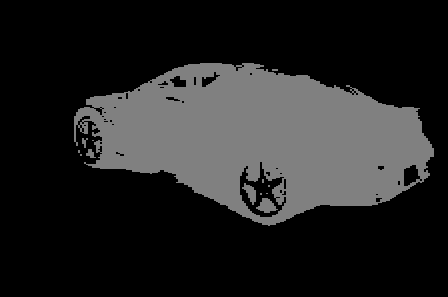
\includegraphics[width=0.20\textwidth,height=0.20\textwidth]
      {figures/val_labels/ours/2010_005119_[6]}        \\



      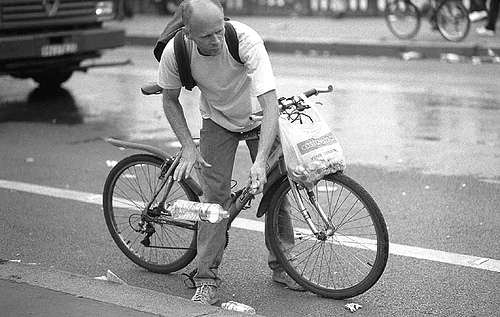
\includegraphics[width=0.20\textwidth,height=0.20\textwidth]
      {figures/originals/2011_000453}
                &
      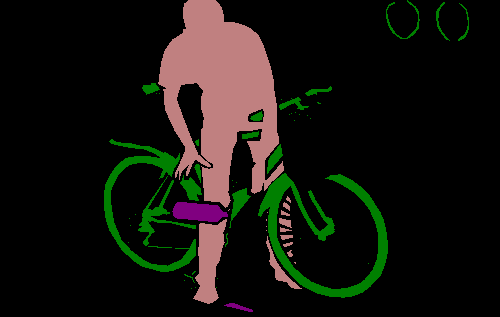
\includegraphics[width=0.20\textwidth,height=0.20\textwidth]
      {figures/colored_gts/2011_000453}
                &
      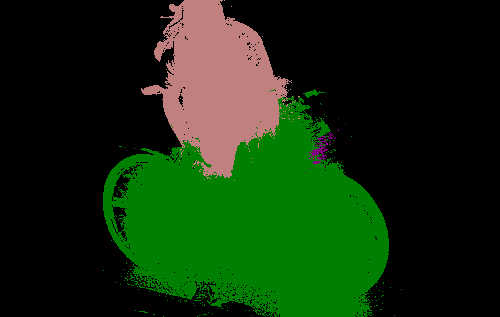
\includegraphics[width=0.20\textwidth,height=0.20\textwidth]
      {figures/val_labels/weclip/2011_000453_[1, 4, 14]}
                &
      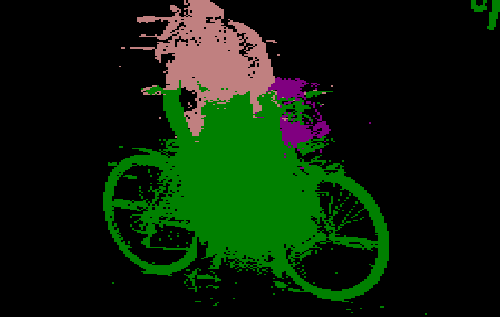
\includegraphics[width=0.20\textwidth,height=0.20\textwidth]
      {figures/val_labels/ours/2011_000453_[1, 4, 14]} \\
    \end{tabular}

    \caption{Qualitative comparison of pseudo-labels between WeCLIP and our UniCL-AffSeg on PASCAL VOC 2012 \textit{val} set.}
    \label{fig:qualitative_comparison_pseudolabel_val}
  \end{tcolorbox}
\end{figure}


\begin{figure}[ht]
  \centering
  \setlength{\tabcolsep}{2pt} % adjust spacing
  \renewcommand{\arraystretch}{0.9}
  % Wrap the table in a colored box (requires \usepackage{tcolorbox})
  \begin{tcolorbox}[colframe=black!60, colback=white, boxrule=0.8pt, arc=2pt, left=2pt, right=2pt, top=2pt, bottom=2pt]
    \centering
    \begin{tabular}{cccc}
      (a) Input & (b) GT & (c) WeCLIP & (d) (Ours)           \\
      [1mm]

      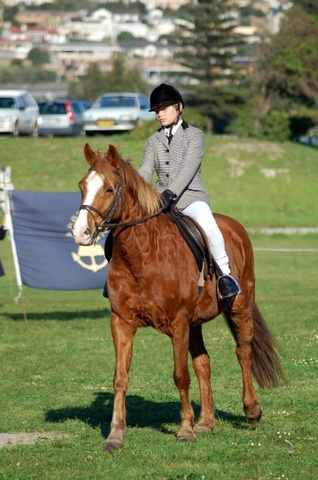
\includegraphics[width=0.20\textwidth,height=0.20\textwidth]
      {figures/originals/2007_005331}
                &
      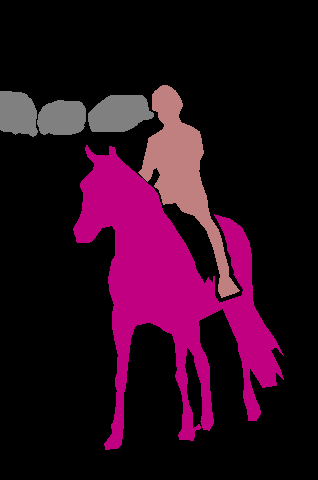
\includegraphics[width=0.20\textwidth,height=0.20\textwidth]
      {figures/colored_gts/2007_005331}
                &
      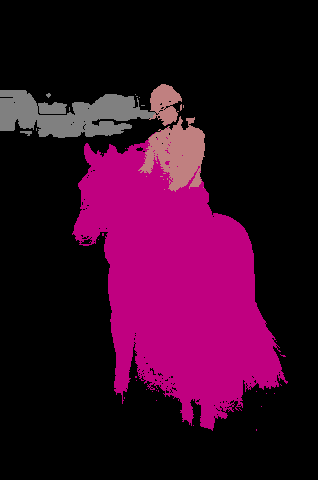
\includegraphics[width=0.20\textwidth,height=0.20\textwidth]
      {figures/test_labels/weclip/2007_005331_[6, 12, 14]}
                &
      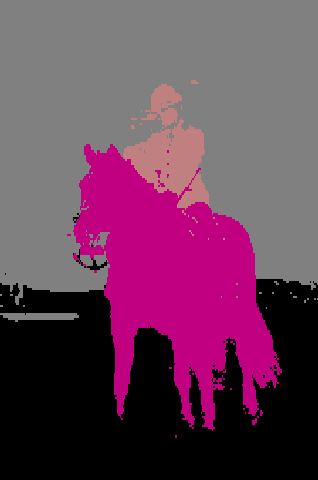
\includegraphics[width=0.20\textwidth,height=0.20\textwidth]
      {figures/test_labels/ours/2007_005331_[6, 12, 14]}    \\

      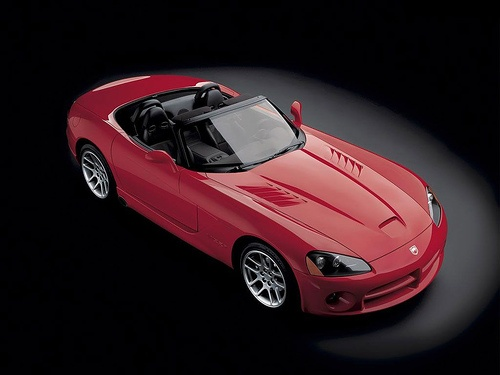
\includegraphics[width=0.20\textwidth,height=0.20\textwidth]
      {figures/originals/2007_006277}
                &
      \includegraphics[width=0.20\textwidth,height=0.20\textwidth]
      {figures/colored_gts/2007_006277}
                &
      \includegraphics[width=0.20\textwidth,height=0.20\textwidth]
      {figures/test_labels/weclip/2007_006277_[6]}
                &
      \includegraphics[width=0.20\textwidth,height=0.20\textwidth]
      {figures/test_labels/ours/2007_006277_[6]}   \\

      \includegraphics[width=0.20\textwidth,height=0.20\textwidth]
      {figures/originals/2008_001504}
                &
      \includegraphics[width=0.20\textwidth,height=0.20\textwidth]
      {figures/colored_gts/2008_001504}
                &
      \includegraphics[width=0.20\textwidth,height=0.20\textwidth]
      {figures/test_labels/weclip/2008_001504_[14]}
                &
      \includegraphics[width=0.20\textwidth,height=0.20\textwidth]
      {{figures/test_labels/ours/2008_001504_[14]}}        \\


      \includegraphics[width=0.20\textwidth,height=0.20\textwidth]
            {figures/originals/2008_002358}
                &
      \includegraphics[width=0.20\textwidth,height=0.20\textwidth]
      {figures/colored_gts/2008_002358}
                &
      \includegraphics[width=0.20\textwidth,height=0.20\textwidth]
      {figures/test_labels/weclip/2008_002358_[0]}
                &
      \includegraphics[width=0.20\textwidth,height=0.20\textwidth]
      {figures/test_labels/ours/2008_002358_[0]}    \\


      \includegraphics[width=0.20\textwidth,height=0.20\textwidth]
      {figures/originals/2009_003224}
                &
      \includegraphics[width=0.20\textwidth,height=0.20\textwidth]
      {figures/colored_gts/2009_003224}
                &
      \includegraphics[width=0.20\textwidth,height=0.20\textwidth]
      {figures/test_labels/weclip/2009_003224_[1]}
                &
      \includegraphics[width=0.20\textwidth,height=0.20\textwidth]
      {figures/test_labels/ours/2009_003224_[1]}        \\



      \includegraphics[width=0.20\textwidth,height=0.20\textwidth]
      {figures/originals/2009_004084}
                &
      \includegraphics[width=0.20\textwidth,height=0.20\textwidth]
      {figures/colored_gts/2009_004084}
                &
      \includegraphics[width=0.20\textwidth,height=0.20\textwidth]
      {figures/test_labels/weclip/2009_004084_[2]}
                &
      \includegraphics[width=0.20\textwidth,height=0.20\textwidth]
      {figures/test_labels/ours/2009_004084_[2]} \\

      
      \includegraphics[width=0.20\textwidth,height=0.20\textwidth]
      {figures/originals/2010_002531}
                &
      \includegraphics[width=0.20\textwidth,height=0.20\textwidth]
      {figures/colored_gts/2010_002531}
                &
      \includegraphics[width=0.20\textwidth,height=0.20\textwidth]
      {figures/test_labels/weclip/2010_002531_[7, 17]}
                &
      \includegraphics[width=0.20\textwidth,height=0.20\textwidth]
      {figures/test_labels/ours/2010_002531_[7, 17]} \\


    \end{tabular}

    \caption{Qualitative comparison of pseudo-labels between WeCLIP and our UniCL-AffSeg on PASCAL VOC 2012 \textit{test} set.}
    \label{fig:qualitative_comparison_pseudolabel_test}
  \end{tcolorbox}
\end{figure}


\subsection{Observations}

\subsubsection{Class Activation Maps (CAMs)}
Our UniCL-AffSeg CAMs demonstrate superior performance compared to WeCLIP in several key aspects:
\begin{itemize}
    \item \textbf{Enhanced Object Coverage and Completeness}: UniCL-AffSeg CAMs exhibit more contiguous and complete activation regions. For instance, in images such as \texttt{2007\_003778\_7.jpg} (cat) and \texttt{2011\_000453\_1.jpg} (bicycle), our CAMs capture larger, more holistic object areas, reducing sparsity and better approximating full object extents. This is attributed to the Swin-based affinity refinement, which effectively propagates activations across object parts.
    \item \textbf{Reduced Background Noise and Sharper Boundaries}: WeCLIP CAMs often include extraneous background activations, leading to noisy and diffuse maps (e.g., in \texttt{2010\_005119\_6.jpg} for car and \texttt{2010\_000148\_5.jpg} for bus). In contrast, UniCL-AffSeg CAMs show cleaner, more focused activations with sharper edges, minimizing false positives. This highlights the benefits of multi-modal fusion in UniCL over WeCLIP's ViT-only approach.
    \item \textbf{Improved Handling of Complex or Small Objects}: For challenging cases like \texttt{2011\_000145\_15.jpg} (pottedplant) and \texttt{2010\_003599\_3.jpg} (boat), UniCL-AffSeg CAMs provide finer granularity and better localization, capturing subtle details that WeCLIP misses. This is evident in multi-class images (e.g., \texttt{2007\_005702\_1.jpg}), where our method separates classes more effectively.
    \item \textbf{Consistency Across Datasets}: These improvements are consistent across both validation and test sets, with examples like \texttt{2007\_005331\_[6, 12, 14].jpg} demonstrating robustness in cluttered scenes.
\end{itemize}

\subsubsection{Pseudo-Labels}
The pseudo-labels generated by UniCL-AffSeg show marked improvements over WeCLIP, aligning more closely with ground truth annotations:
\begin{itemize}
    \item \textbf{Higher Mask Accuracy}: UniCL-AffSeg pseudo-labels capture object shapes more precisely, with fewer misclassifications or holes. For example, in \texttt{2007\_003778\_[7, 15].png} (cat and person), our masks outperform WeCLIP's fragmented outputs.
    \item \textbf{Finer Boundary Delineation}: Our pseudo-labels exhibit cleaner, more defined edges, reducing noise and over-segmentation. In test examples like \texttt{2008\_001504\_[14].png} (horse) and \texttt{2009\_003224\_[1].png}, WeCLIP produces noisy masks, while UniCL-AffSeg yields smoother, more accurate boundaries.
    \item \textbf{Better Performance on Diverse Scenarios}: Trends hold for easy (e.g., \texttt{2011\_001967\_[2].png} for bird) and hard cases (e.g., \texttt{2010\_005119\_[6].png} for car), with UniCL-AffSeg narrowing the gap to fully supervised methods. Limitations persist for highly occluded or tiny objects (e.g., \texttt{2007\_000250\_[4, 10].png}).
    \item \textbf{Cross-Set Generalization}: Similar gains are observed in test labels, such as \texttt{2009\_004084\_[2].png}, underscoring boundary precision and completeness.
\end{itemize}

Overall, these qualitative results underscore UniCL-AffSeg's advantages in weakly supervised semantic segmentation, driven by its Swin transformer backbone and affinity-based refinement. This supports the quantitative improvements (e.g., higher mIoU) reported in the results section, demonstrating UniCL-AffSeg's potential to bridge the gap with fully supervised approaches.



